\documentclass[10pt,conference,compsocconf]{IEEEtran}

%\usepackage{times}
%\usepackage{balance}
\usepackage{url}
\usepackage{graphicx}	% For figure environment
\usepackage{textgreek}
\usepackage{amsbsy}
\usepackage{cleveref}

\begin{document}
\title{Image Compression by Encoding and Single Basis Reconstruction}

\author{
  Pascal Widmer, Julian Fuchs, Stefan Blumer\\
  10-924-439; 10-927-200; 11-921-749\\
  Department of Computer Science, ETH Zurich, Switzerland
}

\maketitle

\begin{abstract}
In the last decade, the amount, size and quality of images was ever increasing. This development makes image compression indispensable. A novel solution for image compression is proposed in this paper. By refining the PCA compression algorithm and introducing a new encoding scheme, images are compressed to a fraction of their original size while still maintaining image quality. The proposed algorithm is compared to other baseline image compression algorithms.
\end{abstract}

\section{Introduction}
Image compression is a fundamental step in distributing images. In fact, most images found are compressed. The two most widely encountered compression algorithms are PNG (Portable Network Graphics), which supports lossless image compression and JPEG, which implements lossy image compression. Another very well known lossy image compression algorithm uses PCA (Principal Component Analysis) for patches.
\\
\\
In this paper, we refine the latter algorithm. Recognizing the fact that in a color image, the color channels red, green and blue are often very similar, led us to a new compression scheme, described in this paper. We also propose a new encoding method to further improve our compression. The compression algorithm proposed in this paper achieves a compression rate of 1.6\% with a mean error of 0.0014. This means that we compress an average image to roughly 2\% of its original size, while still maintaining a relatively small difference to the original file.
\subsection{Related Works}
Improvements to PCA has been done by Jieping Ye, Ravi Janardan and Qi Li~\cite{neural} who concentrated their efforts on image recognition. Image compression by means of PCA combined with neural networks learning was done by S.Costa and S.Fiori~\cite{GPCA}.
\section{Models and Methods}
The goal of image compression is to compress a given image to the smallest size possible while the reconstructed image from the compression has the smallest error possible. The proposed compression algorithm in this paper works on jpg files of any size.
\begin{figure}[h!]
\centering
  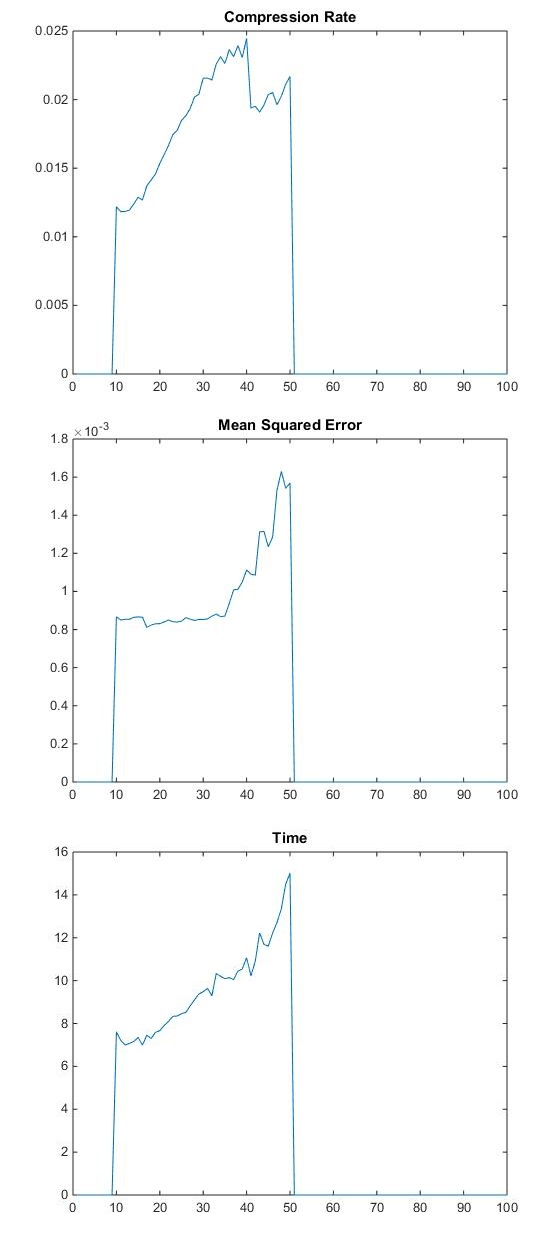
\includegraphics[scale=0.4]{figures/DsCombined2.jpg}
  \caption{Time, mean squared error and compression rate for different choices of patch sizes \textbf{d} for the Lena standard test image}
  \label{fig:DS}
\end{figure}
\subsection{Compression}
As a first step in our compression algorithm, the initial image is transformed into a patch representation in a process called \textit{feature extraction}. The image is split into patches of length and  width \textbf{d}. If the length or width of the image is not dividable by \textbf{d}, we pad the image with as many last rows/columns as necessary to be able to divide the image into patches of size \textbf{d}*\textbf{d}. For a colored image, this process is done for each color channel red, green and blue separately. In the case of a grayscale image, the process is only applied once. We chose \textbf{d} to be 10 based on a study on example images. In \Cref{fig:DS}, the time, mean squared error and compression rate are shown for each patch size \textbf{d} for the Lena standard test image.
\\
\\
In the following, we assume the image is grayscale and we will treat the case of colored images later on. After having split the grayscale image into patches, we reinterpret the image as a matrix $\boldsymbol{\Gamma}$ with the patches as its columns. Computing the covariance matrix of $\boldsymbol{\Gamma}$ returns the matrix  $\boldsymbol{\Sigma}$. We apply the eigendecomposition on $\boldsymbol{\Sigma}$, which returns a matrix \textbf{U} containing the eigenvectors and a diagonal matrix $\boldsymbol{\Lambda}$ containing the associated eigenvalues. A function is run which analyses the eigenvalues and returns the number of eigenvalues \textbf{k} which make up 99\% of the sum of all eigenvalues. Selecting the eigenvectors corresponding to the \textbf{k} largest eigenvalues, a basis \textbf{Uk} is found in which we express $\boldsymbol{\Sigma}$. This is done by the simple matrix multiplication of \textbf{Uk} and $\boldsymbol{\Gamma}$ which results in a matrix \textbf{Z}. Our compression consists of \textbf{Z} and \textbf{Uk} and some settings used for the reconstruction.
\\
\\
As mentioned before, a color image is split into a separate matrix for each color channel red, green and blue. Again taking the Lena standard test image as an example, we see that the three channels red, green and blue are in fact very similar, as seen in \Cref{fig:Lena}. This discovery led us to the idea to express the color channels red, green and blue in the same basis. For each of the color channels we find a basis with the algorithm explained above. From the red, green and blue basis we select the one basis which has the least mean squared error for our compression. The compression for a colored image then consists of the coefficient matrices for red, green and blue and the chosen basis.
\begin{figure}[h!]
\centering
  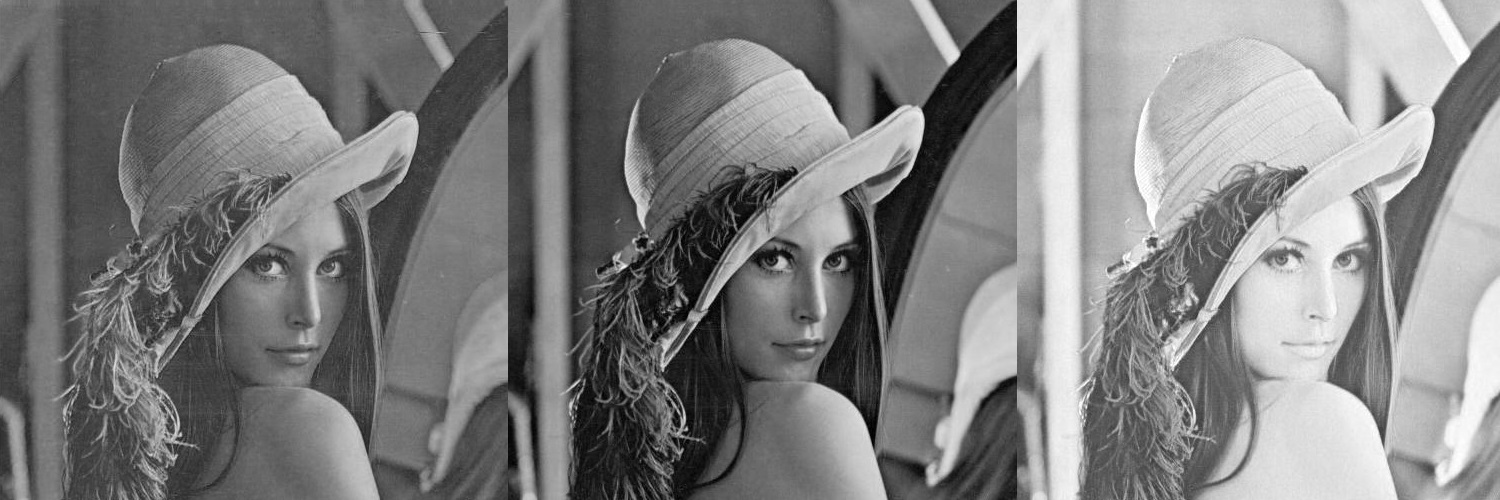
\includegraphics[scale=0.21]{figures/LenaCombined.jpg}
  \caption{The 3 color channels red, green and blue for the Lena standard test image}
  \label{fig:Lena}
\end{figure}
\subsection{Encoding}
The matrices, which initially contain double values, are further compressed by encoding them in a custom binary format. The common double-precision floating-point format allocates 1 sign bit, 11 exponent bits and 52 fraction bits for each matrix entry. We make use of the fact that values stored in our matrices are of the same order of magnitude and thus not all exponent bits are needed. Furthermore, most of the 52 fraction bits contribute little to the measured compression error and are simply discarded. Values which are close to 0.0, i.e., have an absolute value which lies in some interval [0, $\epsilon$], are rounded to 0.0. They are handled as special cases and can be encoded with only 1 bit. We end up with a binary stream containing some parameters in the first 64 bits including the number of fraction and exponent bits we kept and the new exponent bias followed by a stream of encoded matrix values. An encoded value is either a single bit set to 1 signifying 0.0 or a block of bits where the first bit is 0 followed by the sign flag and the new exponent and fraction bits. In our work we decided to set epsilon to 0.15 while only keeping 5 fraction bits. This way a compression rate of around 0.05 is achieved.
\subsection{Decompression}
After decoding and reading the coefficient matrices for red, green and blue or grayscale and the basis \textbf{Uk} used in the compression, the restoration of the image is simple. For each coefficient matrix \textbf{Z} we calculate the matrix multiplication \textbf{Uk} * \textbf{Z}. The resulting matrix $\boldsymbol{\Xi}$ contains the reconstructed image in its feature extracted form, i.e, the patches are stored in its columns. We simply have to rewrite the values in the columns of $\boldsymbol{\Xi}$ to the patches in the image. In a last step we have to remove the rows and columns we padded the image with in the compression phase.
\\
\\
If the image has color, we repeat this process for each color channel red, green and blue and concatenate the 3 matrices into a three dimensional matrix. If the image is grayscale, the process is only done once.
\section{Results and Discussion}
In \Cref{fig:Comp} a comparison can be found between the algorithm proposed in this paper, the baseline PCA algorithm on patches and the image compression algorithm using Haar wavelets on the Lena standard test image. We can establish that taking considerably more time than the other two algorithms is well worth it. The mean squared error is significantly lower while maintaining an astonishingly small compression rate. Our algorithm compresses an image to about 1\% of its original size while conserving the image with a minimal error.
\\
\\
Computing the average mean squared error and compression rate for each of the three algorithms, we get:
\begin{table}[h!]
\begin{center}
 \begin{tabular}{||c c c c||} 
 \hline
 Algorithm & Avg. Quad. Error & Avg. Compr. Rate\\ [0.5ex] 
 \hline\hline
 Project & 0.0014 & 0.016\\ 
 \hline
 PCA standard & 0.0142 & 0.083\\
 \hline
 Haar wavelet & 0.0015 & 0.0418\\
 \hline
\end{tabular}
\end{center}
\end{table}
\\
\\
\begin{figure}[h!]
\centering
  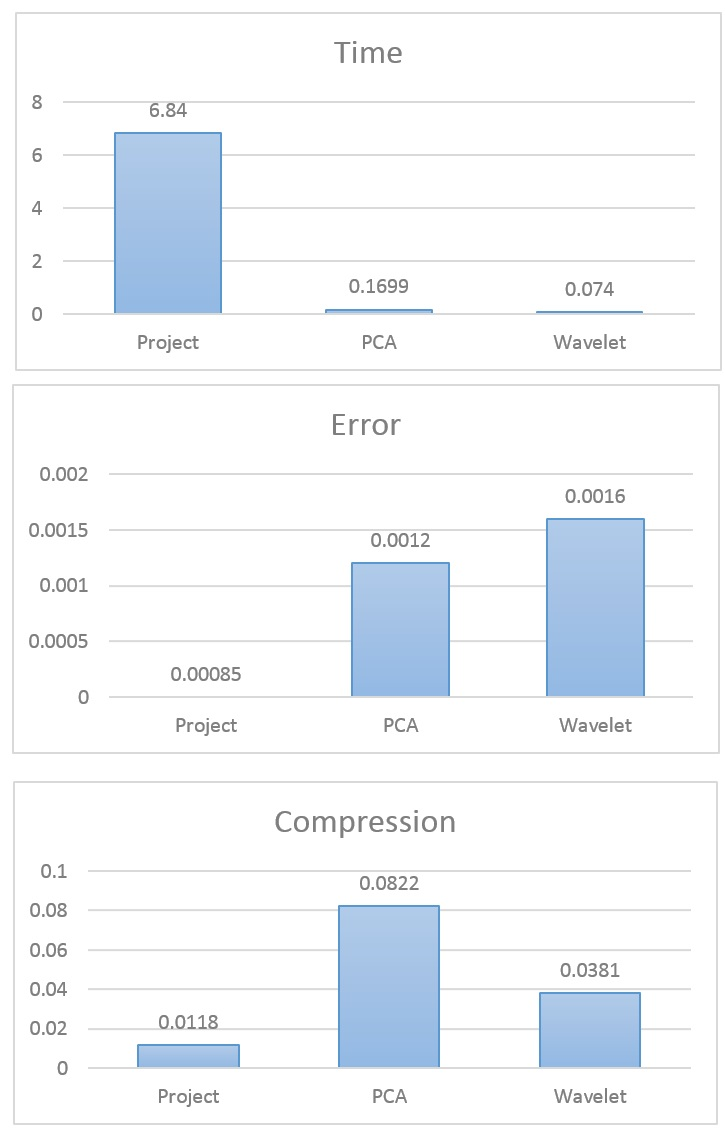
\includegraphics[scale=0.4]{figures/Comparison.jpg}
  \caption{Comparison between the algorithm proposed in this paper, the regular PCA algorithm and the algorithm for image compression using Haar wavelets. The comparison was done on the Lena standard test image. The time table was measured in seconds, the error table shows the mean squared error of the reconstructed image and the compression table shows the compression rate of each algorithm}
  \label{fig:Comp}
\end{figure}
\section{Summary}
We proposed a novel solution for image compression by refining the PCA compression algorithm. We realized that the color channels of a colored image are similar. Our approach was to represent the three color channels in single basis, minimizing the compression with only a diminishing increase of the error of the reconstructed image. We developed an algorithm choosing the best base and the best size of that base. An introduced encoding scheme further improves our compression rate significantly, resulting in a substantial improvement to the PCA image compression algorithm.
\bibliographystyle{IEEEtran}
\bibliography{groupLightRain-references}
  
\end{document}

